\section{Improving CNN Training}
\subsection{Underfitting}

\subsubsection{Batch Normalization}



\begin{wrapfigure}{r}{4cm}%靠文字内容的右侧
	
	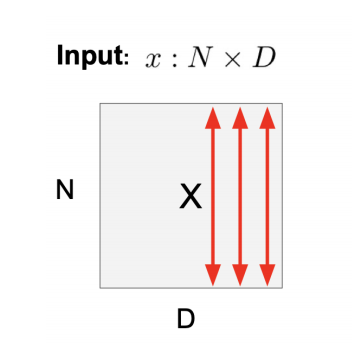
\includegraphics[scale=0.65]{figures/BNsize.png}
	\caption{Input of Batch Normalization}
	\label{Input of Batch Normalization}
	
\end{wrapfigure}

所谓Batch Normalization,中文译名为"批标准化".其基本操作是在进入激活函数层之前,将数据逐通道进行标准化.假设输入为$n$个数据,通道数为$D$,如右图.

那么我们需要计算
\begin{equation}
	\begin{split}
		\mu_j &= \frac{1}{N} \sum_{i=1}^{N} x_{i, j}
		\\
		\sigma_j^2 &= \frac{1}{N} (x_{i, j} - \mu_j)^2
		\\
		\hat{x}_{i, j} &= \frac{x_{i, j} - \mu_j}{\sqrt{\sigma_j^2 + \epsilon}}
	\end{split}
	\label{BN calculation}
\end{equation}
其中$\epsilon$是为防止方差为$0$而添加的小量.这一步是标准化的过程,此层还需要进行一步处理:
\begin{equation}
	y_{i, j} = \gamma_{j} \hat{x}_{i,j} + \beta_j
\end{equation}
我们需要学习$\gamma, \beta$这两个$D$维参数.

那么,为什么要进行BN操作呢?

在机器学习领域有个很重要的假设:独立同分布假设,就是假设训练数据和测试数据是满足相同分布的,这是通过训练数据获得的模型能够在测试集获得好的效果的一个基本保障.那BatchNorm的作用是什么呢?BatchNorm的作用就是在深度神经网络训练过程中使得每一层神经网络的输入保持相同分布.

对于深度学习这种包含很多隐层的网络结构,在训练过程中,因为各层参数不停在变化,所以每个隐层都会面临covariate shift的问题,也就是在训练过程中,隐层的输入分布经常发生变化,这就是所谓的“Internal Covariate Shift”,Internal指的是深层网络的隐层,是发生在网络内部的事情.

BatchNorm的基本思想就是:能不能让每个隐层节点的激活输入分布固定下来呢?这样就避免了“Internal Covariate Shift”问题了.

之前的研究表明如果在图像处理中对输入图像进行白化操作的话——所谓白化,就是对输入数据分布进行PCA,并将各个分量变换到0均值,单位方差的正态分布——那么神经网络会较快收敛.但是白化操作较难进行,而且操作不可导.而BN可以理解为对深层神经网络每个隐层神经元的激活值做简化版本的白化操作.

BN的基本思想其实相当直观:因为深层神经网络在做非线性变换前的激活输入值随着网络深度加深或者在训练过程中,其分布逐渐发生偏移或者变动,之所以训练收敛慢,一般是整体分布逐渐往非线性函数的取值区间的上下限两端靠近(对于Sigmoid函数来说,意味着激活输入值是大的负值或正值),所以这导致反向传播时低层神经网络的梯度消失,这是训练深层神经网络收敛越来越慢的本质原因,而BN就是通过一定的规范化手段,把每层神经网络任意神经元这个输入值的分布强行拉回到均值为0方差为1的标准正态分布,其实就是把越来越偏的分布强制拉回比较标准的分布,这样使得激活输入值落在非线性函数对输入比较敏感的区域,这样输入的小变化就会导致损失函数较大的变化,意思是这样让梯度变大,避免梯度消失问题产生,而且梯度变大意味着学习收敛速度快,能大大加快训练速度.

对于每个隐层神经元,把逐渐向非线性函数映射后向取值区间极限饱和区靠拢的输入分布强制拉回到均值为0方差为1的比较标准的正态分布,使得非线性变换函数的输入值落入对输入比较敏感的区域,以此避免梯度消失问题.

以上关于BN基本思想的叙述来自参考文献\cite{BN}.但是在BN原论文\cite{BNpaper}当中,作者也提出了只进行 \ref{BN calculation} 的问题:它可能限制模型的表达能力.以Sigmoid为例,标准化将所有的输入集中于$0$附近,而这里正是Sigmoid的线性近似区域,这样Sigmoid层的作用就和线性层类似了.因此BN需要再加一项平移和拉伸,并把这两项参数作为学习对象.

总之,BatchNorm的提出试图通过标准化解决深层神经网络当中内部协变量漂移的问题,将数据限制在一定范围内,并通过平移和拉伸操作减少此操作对模型表达能力的影响.但是,后来有人提出了新的看法:BatchNorm对ICS的减缓微乎其微,它是通过平滑化loss landscape来起到作用的.

但BatchNorm有一点需要额外注意:那就是在测试集上运行时,BatchNorm层并不是计算输入的期望方差,而是调用在训练时储存的$\mu, \sigma$.具体来说,按照以下方式迭代每次运算得到的$\mu_{rms}$:
\begin{equation}
	\begin{cases}
		\mu_{rms}^\prime = \rho \mu_{rms} + (1-\rho) \mu_t 
		\\
		\sigma_{rms}^\prime = \rho \sigma_{rms} + (1-\rho) \sigma_t 
	\end{cases}
\end{equation}

BatchNorm通常位于FC层或Conv层之后,非线性层之前.它有如下的优点:

\begin{enumerate}
	\item 使得深层网络更加容易训练,因为它可以减缓梯度消失.
	\item 允许使用更大的学习率,并且收敛更快.这是因为如果不加BatchNorm,则深层网络容易产生级联效应,学习率如果比较大,则前面的layer发生变化将会引起后面的层的剧烈变化,极不稳定.
	\item 网络对于参数的初始化要求降低,因为会进行标准化操作.
	\item Act as regularization during training.?
	\item 测试时不花费开销,可与Conv一同使用
\end{enumerate}

但是同时需要注意:BatchNorm在训练和测试时行为不同!这是Bug的一个常见原因.此外,一旦使用了BatchNorm,那么Batch就不能太小,否则会使$\mu, \sigma$变得极不稳定,这可能会导致模型在训练集和测试集上的性能的巨大差异.

\begin{figure}[htbp]
	\centering
	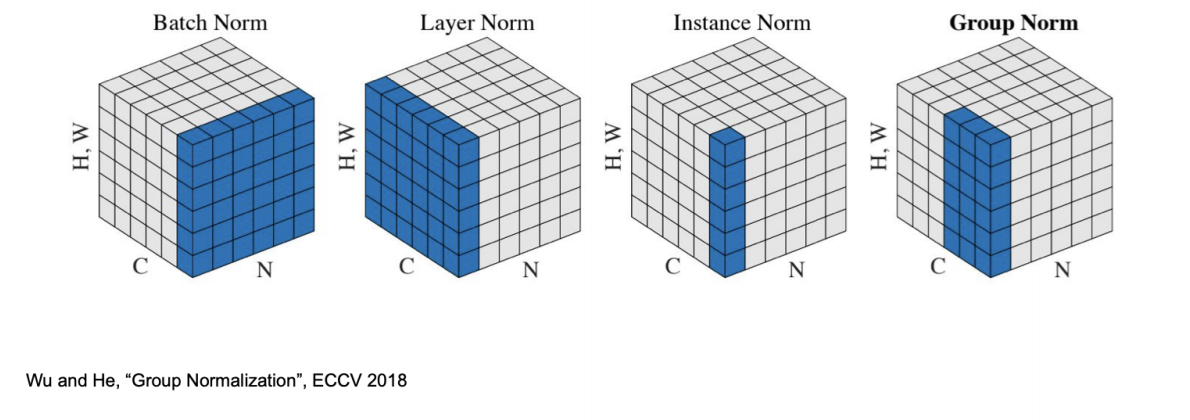
\includegraphics[scale=0.55]{figures/NormalizationTechniques.png}
	\caption{NormalizationTechniques}
	\label{fournorm}
\end{figure}

这样的特性使得人们自然而然提出了一个问题:我们能否绕过BatchSize的限制?如果可行,那么就不会存在训练和测试的差异.

图 \ref{fournorm} 当中的$C,N$分别代表通道数和样本数,$H,W$等维度因为地位相同,被压缩为一个维度,可以视为图片的宽和高.左一逐通道对所有样本求平均值,正是BatchNorm.要想脱离BatchSize的限制,就必须不沿$N$方向处理.

左二是对$C,H,W$三个维度求平均,这其实蕴含了所有数据服从同一分布的假设,但实际上可能并非如此.比如,偏绿色的图片在$G$通道上的$\mu$更高,这样做会破坏不同channel的差异性,效果比BatchNorm更差,因此极少应用于CV领域,但在NLP领域应用广泛.

右二其实就对应了BatchSize=1的情形,其问题前文已述.虽然其存在巨大的不稳定性,但其$\mu, \sigma$表征了图片风格,因此在Style Transfer当中常用.

\begin{wrapfigure}{r}{6cm}
	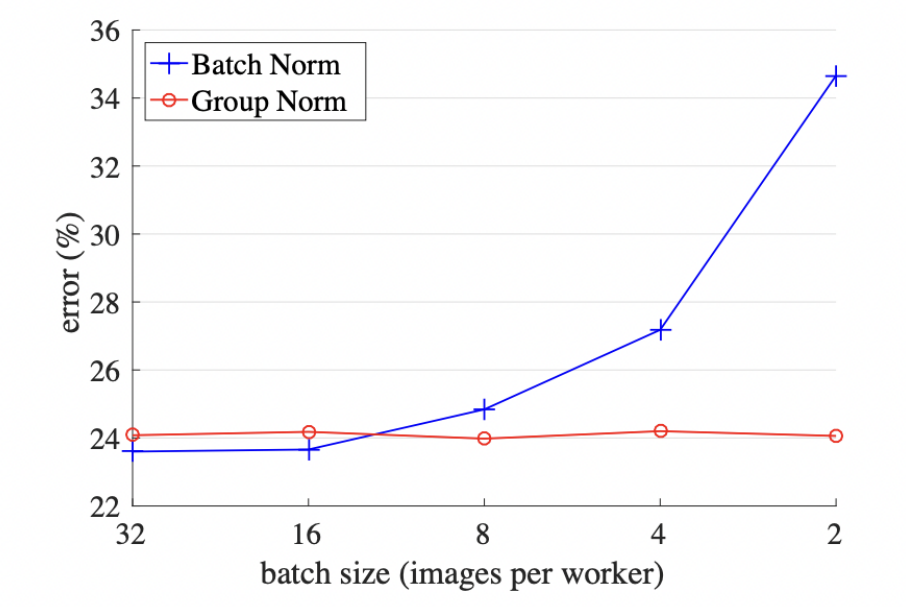
\includegraphics[scale=0.30]{figures/GroupNorm.png}
	\caption{classification error vs batch sizes}
	\label{groupNorm}
\end{wrapfigure}

右一是由何恺明等人提出的GroupNorm,它将channel分组进行计算,相当于对图2和图3进行了插值.

图 \ref{groupNorm}是He在论文中给出的一个ResNet-50模型的训练结果,可以看出在BatchSize较大的时候,BatchNorm表现略优于GroupNorm,但随着BatchSize减小,前者的错误率快速增长,而后者的错误率则没有明显变化.当训练集的BatchSize不得不很小或Batch之间差异极大时,应该选用GroupNorm.


\subsubsection{ResNet or Skip Links}
介绍BatchNorm之后,CNN网络结构可修改如下:
$$\texttt{[(Conv-BN-ReLu)*N-Pool?]*M-(FC-BN-ReLu)*K-FC-SoftMax}$$

注意最后的\texttt{FC-SoftMax}之间无需添加\texttt{BN}.那么,层数是越深越好吗?我们来看下图.
\begin{figure}[htbp]
	\centering
	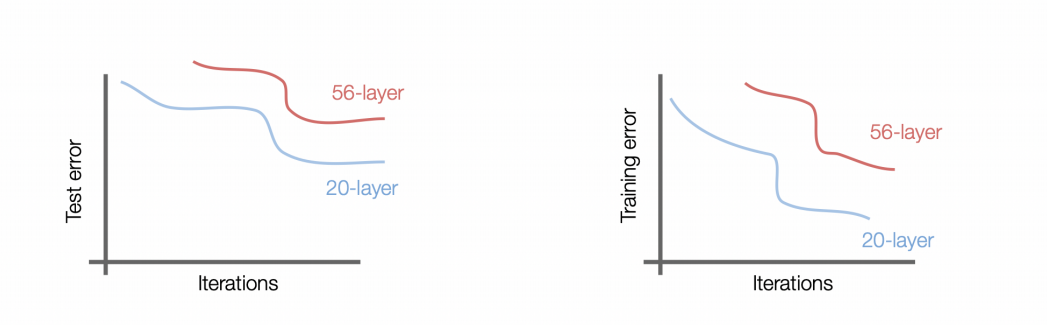
\includegraphics[scale=0.65]{figures/deep-test-err.png}
	\caption{两种深度的神经网络的测试误差(左)和训练误差(右)}
	\label{过拟合}
\end{figure}

56层神经网络在测试集上误差大于20层,我们可以解释为是过拟合导致,但其在训练集上的误差竟然也更大,这就说明更深的神经网络表现不佳并不是过拟合导致.那么在CNN变深的过程中,究竟产生了什么问题呢?

现在的事实是:更深的模型具有更强的表达能力(即更多参数),但是表现却更差.我们提出一个假设:可能是因为深层的神经网络更加难以进行优化.这个时候我们应该控制变量找出原因.\footnote{在接下来将较浅层的输出通过一条旁路直连深层的操作,老师称之为"寻找一种中间状态",即将浅层网络加上恒等变换层"视为"深层网络,再将两个进行叠加.}一种让深层网络至少和浅层网络一样好的方法是,将浅层网络加上一些恒等变换的层,"变成"深层网络.从这种意义上看,更深的网络不应该比浅的差,只要中间的一些层学习成恒等变换即可.这可能预示着,对于深层网络而言,"恒等"是一个较难学习的特征.这或许是因为深层网络引入太多非线性表达,在高维的参数空间中难以学习到恒等吧.\footnote{本小节余下的内容取自\cite{WhyResNetWorks}.}

\begin{wrapfigure}{r}{4cm}
	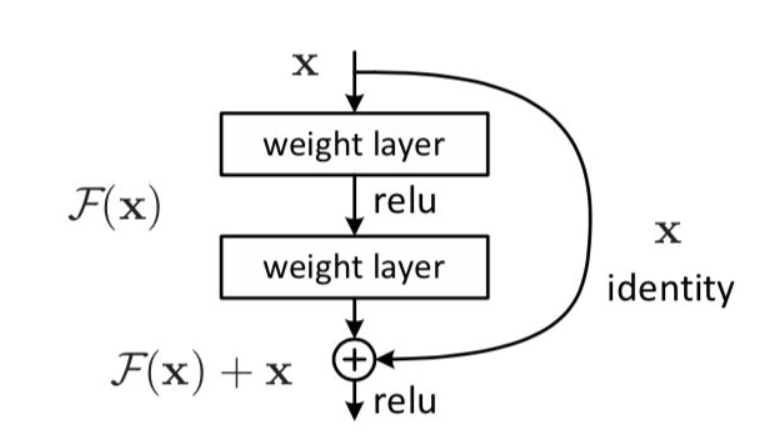
\includegraphics[scale=0.35]{figures/residual_network.png}
	\caption{残差神经网络单元}
\end{wrapfigure}

既然如此,那么一种自然的思路就是:构造天然的恒等.假设神经网络非线性层的输入输出维度一致,那么可以将要拟合的函数分成两个部分:
\begin{equation}
	\mathbf{z}^{(l)}=\mathcal{H}\left(\mathbf{a}^{(l-1)}\right)=\mathbf{a}^{(l-1)}+\mathcal{F}\left(\mathbf{a}^{(l-1)}\right)
	\label{残差神经网络表达式}
\end{equation}

其中 $\mathcal{F}(\cdot)$ 是残差函数.在网络高层,学习一个恒等映射 $\mathcal{H}\left(\mathbf{a}^{(l-1)}\right) \rightarrow \mathbf{a}^{(l-1)}$ 即等价于令残差部分趋 近于0,即 $\mathcal{F}\left(\mathbf{a}^{(l-1)}\right) \rightarrow \mathbf{0}$ .
残差单元可以以跳层连接的形式实现,即将单元的输入直接与单元输出加在一起,然石再激活.因 此残差网络可以轻松地用主流的自动微分深度学习框架实现,直接使用BP算法更新参数.

实验表明,残差网络很好地解决了深度神经网络的退化问题,并在ImageNet和CIFAR-10等图像任务上取得了非常好的结果,同等层数的前提下残差网络也收敛得更快.这使得前馈神经网络可以采用更深的设计.除此之外,去除个别神经网络层,残差网络的表现不会受到显著影响,这与传统的前馈神经网络大相径庭.

那么,残差神经网络为什么有效呢?

从梯度反向传播的角度,Skip Link提供了一条梯度反向传播的旁路,使得梯度可以更加顺畅地传递到浅层.我们考虑式 \ref{残差神经网络表达式} 描述的层,假设残差块不采取任何激活函数,即
\begin{equation}
	\bold{a}^{(l)} = \bold{z}^{(l)}
\end{equation}

考虑$l_1>l_2$两个层,递归地进行展开,有
\begin{equation}
	\mathbf{a}^{\left(l_{2}\right)}=\mathbf{a}^{\left(l_{1}\right)}+\sum_{i=l_{1}}^{l_{2}-1} \mathcal{F}\left(\mathbf{a}^{(i)}\right)
\end{equation}

在前向传播时,输入信号可以从任意低层直接传播到高层.由于包含了一个天然的恒等映射,一定程度上可以解决网络退化问题.
这样,最终的损失函数$\mathcal{L}$对某低层输出的梯度可以展开为
\begin{equation}
	\frac{\partial \mathcal{L}}{\partial \mathbf{a}^{\left(l_{1}\right)}}=\frac{\partial \mathcal{L}}{\partial \mathbf{a}^{\left(l_{2}\right)}}+\frac{\partial \mathcal{L}}{\partial \mathbf{a}^{\left(l_{2}\right)}} \frac{\partial}{\partial \mathbf{a}^{\left(l_{1}\right)}} \sum_{i=l_{1}}^{l_{2}-1} \mathcal{F}\left(\mathbf{a}^{(i)}\right)
\end{equation}

上式说明,反向传播时,错误信号可以不经过任何中间权重矩阵变换直接传播到低层,一定程度上可以缓解梯度弥散问题(即便中间层矩阵权重很小,梯度也基本不会消失).综上,可以认为残差连接使得信息前后向传播更加顺畅.

在文章 \cite{ResidualNetworksAreExponentialEnsembles} 中,作者提出了另一种观点,认为残差神经网络是由一系列路径集合组装成的模型.

\begin{figure}[htbp]
	\centering
	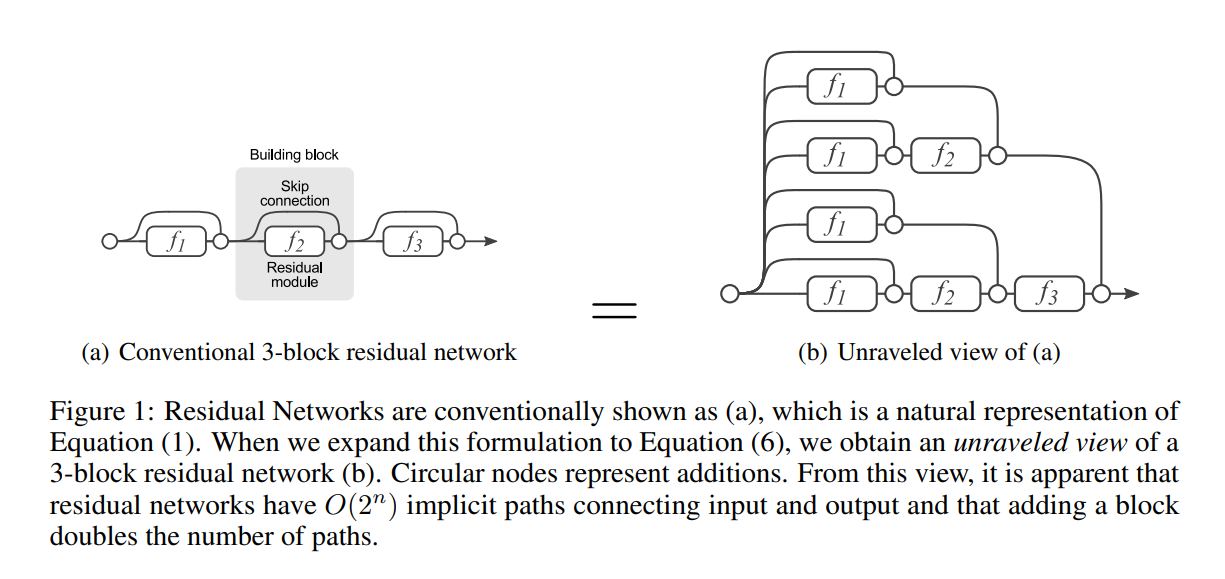
\includegraphics[scale=0.55]{figures/ResNet集成神经网络解释.png}
	\caption{文章给出的配图}
	\label{}
\end{figure}


Andreas Veit等人展开了几组实验,在测试时,删去残差网络的部分网络层(即丢弃一部分路径)、或交换某些网络模块的顺序(改变网络的结构,丢弃一部分路径的同时引入新路径).实验结果表明,网络的表现与正确网络路径数平滑相关(在路径变化时,网络表现没有剧烈变化),这表明残差网络展开后的路径具有一定的独立性和冗余性,使得残差网络表现得像一个集成模型(ensemble).作者还通过实验表明,残差网络中主要在训练中贡献了梯度的是那些相对较短的路径.


\subsection{Overfitting}

过拟合产生的原因是data和model之间的不平等.例如分类问题,我们给网络输入的数据,对于机器来说就是某个概念的"定义".但同类事物有共性也有差别,定义应当只取其共性,但神经网络并不一定能做到这一点.所以,减弱model增强data的手段,有助于打破这种不平衡.

首先我们来看看在神经网络训练过程中常见的generalization gap:
\begin{figure}[htbp]
	\centering
	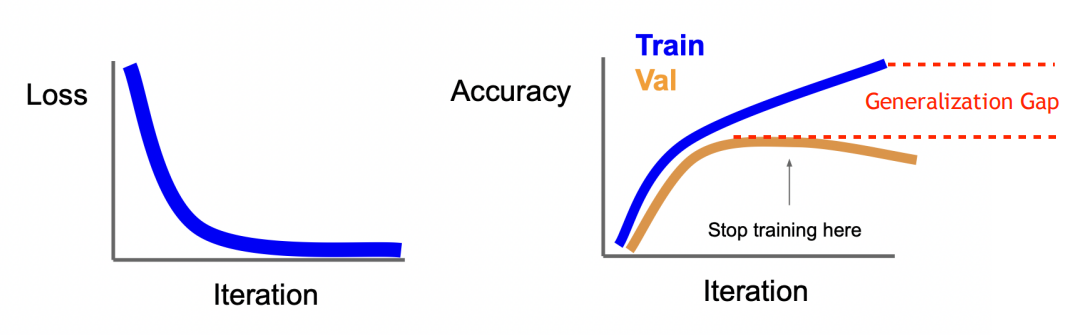
\includegraphics[scale=0.65]{figures/generalgap.png}
	\caption{generalization gap 示意图}
	\label{}
\end{figure}

所谓generalization gap,就是指模型在同分布的训练集和测试集上表现出的准确率差异.这里右图略有瑕疵,我们说的gap应该是指同一轮测试之后两个集合上表现的差异.另外需要注意的是:在训练时即使loss一直在减小,也并不说明在测试集上的准确率在提升,因为可能有过拟合的问题.

对一个过拟合的模型来说,它包含了多于区分数据所必须的数量的参数.为减少过拟合,我们可以从数据和模型两方面着手处理.数据方面,一种自然的想法是,如果训练集数据充足而且包含较多各种无关特征,那么模型更不容易过拟合.最简单的方法是增加数据量,但有时这是代价很大的,我们可以对现有的数据进行处理,获取更多数据.而在模型方面,我们将采取一些限制模型复杂度的处理.数据方面包括Data Augmentation等,而后者我们会提及正则化与Dropout.

\subsubsection{Data Augmentation}

所谓数据增强(data augmentation),就是一种利用已有数据人工生成新数据的手段.常用的手段有翻转(flip),旋转(rotation),缩放(scale),裁剪(crop),移位(translation)和高斯噪声\footnote{当神经网络试图学习可能无用的高频特征(大量出现的模式)时,通常会发生过度拟合.具有零均值的高斯噪声基本上在所有频率中具有数据点,加入图片中可以有效地扭曲高频特征.这也意味着较低频率的组件(通常是预期数据)也会失真,但这种困难可以被克服.}(Gaussian Noise)等.

例如,如果我们的网络需要识别猫的图片,那么在训练时,我们可以将一张图片水平翻转,这当然还是一只猫.于是我们轻松将数据量翻了个倍.

但是!要注意的是,你必须保证\textbf{数据增强之后,你所希望学习的特征并没有发生改变}.这隐含着一种对称性,\sout{而诺特定理指出每种对称性对应一种守恒量,我们不难看出数据增强的依赖的对称性对应的守恒量就是标签...(胡言乱语)}即每一只猫是左右对称的.相对应地,我们很少对猫图片进行上下翻转.所以,进行正确的数据增强是很重要的.比如下面这种反面教材:

\begin{figure}[htbp]
	\centering
	\subfigure[错误的DA]{
		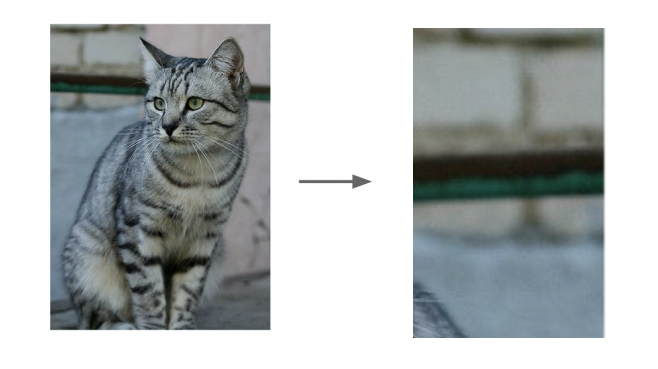
\includegraphics[scale=0.65]{figures/wrongDA.png}
	}
	\subfigure[神经网络直呼我逐渐理解一切]{
		
\includegraphics[scale=0.5]{figures/strangeknowledge.png}
	}
\end{figure}

总之,DA不能太强也不能太弱,很多时候其程度还是需要人工评判.

在空间位置方面的数据增强手段有缩放,裁剪,翻转,填充,旋转,移位,仿射变换(affine transformation)等.色彩方面,可以调整亮度(brightness),对比度(contrast),饱和度(saturation),色调(hue)等.此外还可以应用GAN/RL完成数据增强.

\subsubsection{Regularization}

所谓正则化,就是限制模型复杂度的一种手段.具体做法就是在损失函数当中添加一项正则项:
\begin{equation}
	L(W) = \underbrace{\frac{1}{N}\sum_{i=1}^{N} L_i(f(x_i, W), y_i) }_{Data Loss:\text{模型预测需要拟合训练集}} + \underbrace{\lambda R(W)}_{Regularization:\text{防止模型在训练集上}\textbf{表现太好}}
\end{equation}

举个例子,对于7个散点,我们可以拟合成一条直线,也可以用六次函数经过每一个点,但后者常常不是我们想要的,而正则项的添加就是对模型训练程度的一个限制.设想一个模型是六次函数,我们如何限制其表达近似线性的数据?只需将常数项和一次项系数之外的系数限制在0附近即可.

这种想法与一种哲学原理不谋而合:即Occam's Razar.我们常用的正则函数有$\mathbb L_2$ Regularization: $R(W) = \sum_{k,l}W_{k, l}^2$,以及$\mathbb L_1$ Regularization: $R(W) = \sum_{k,l}\abs{W_{k, l}}$,以及其混合等.使用时需要注意:$\lambda$需要控制正则项的量级,使其与损失函数相当,否则如果正则项过大,会使得网络全力向简单发展;反之则没有效果.

\subsubsection{Dropout}
简单地说,Dropout就是以某个概率随机使神经元失效.

\subsubsection{BatchNorm作为正则化}
BatchNorm使得进入激活函数的输入必须服从特定的高斯分布,这限制了模型的表达能力,因此也是一种正则化的手段,有助于减少过拟合.使用BatchNorm后,就不需要再添加Dropout了.

总之,纵观各种正则化的方法,处处透露出 Less is More 的思想,即越简单的表达方式越好.\footnote{Less is More, but More is different.(笑)}

\subsection{Summary of Mitigating Overfitting}
原则:平衡数据的多样性和模型的容量.

方法:
\begin{enumerate}
	\item Data Augmentation.(从数据的角度)
	\item BatchNorm.(模型角度)
	\item Regularization.(模型角度)
	\item Dropout.(模型角度)
\end{enumerate}

其中DA和BN用了总是比不用好.后两者视情况而定.Dropout一般只用于较大的FC层.